%\section{气体的一维等熵定常流动}
\subsection{气体一维定常流动的基本方程}
\subsubsection{连续性方程}
\begin{frame}{连续性方程}
  %\begin{figure}
  %\begin{tikzpicture}
    %\draw (0,0) .. (3, 1.5);
    %\draw (1.8,0) .. (2.8, 2.5);
  %\end{tikzpicture}
  %\end{figure}
  一维定常可压缩流体的连续性方程:
  \begin{equation*}
    \rho_{1}v_{1}A_{1}
    =
    \rho_{2}v_{2}A_{2}
    \quad
    \mbox{或}
    \quad
    \rho vA=Q=\mathrm{C}
  \end{equation*}
  两边取对数:
  \begin{equation*}
    \ln{\rho} 
    +
    \ln{v}
    +
    \ln{A}
    =
    0
  \end{equation*}
  对上式微分:
  \begin{equation*}
  \frac{\mathrm{d}\rho}{\rho}
  +
  \frac{\mathrm{d}v}{v}
  +
  \frac{\mathrm{d}A}{A}
  =
  0
  \end{equation*}
\end{frame}


\subsubsection{运动方程}
\begin{frame}{运动方程}
  \begin{equation*}
  \frac{\partial u_{x}}{\partial t}
  +
  u_{x}\frac{\partial u_{x}}{\partial x}
  +
  u_{y}\frac{\partial u_{x}}{\partial y}
  +
  u_{z}\frac{\partial u_{x}}{\partial z}
  =
  f_{x}
  -
  \frac{1}{\rho}\frac{\partial p}{\partial x}
  \end{equation*}
  \begin{itemize}
    \item 一维流动:$u_{x}=v$,$u_{y}=u_{z}=0$
    \item 定常流动:$\displaystyle \frac{\partial u_{x}}{\partial t}=0$
    \item 质量力忽略:$f_{x}=0$
  \end{itemize}
  \begin{equation*}
  v \frac{\mathrm{d} v}{\mathrm{d} x}
  =
  -
  \frac{1}{\rho}\frac{\mathrm{d} p}{\mathrm{d} x}
  \end{equation*}
  \begin{equation*}
  v\mathrm{d}v
  +
  \frac{1}{\rho}\mathrm{d}p
  =
  0
  \end{equation*}
  \begin{equation*}
    \int{\frac{1}{\rho}}\mathrm{d}p
    +
    \frac{v^{2}}{2}
    =
    \mathrm{C}
  \end{equation*}
\end{frame}

\subsubsection{能量方程}
\begin{frame}{能量方程}
  热力学第一定律:
  \begin{equation*}
  \mathrm{d}q
  =
  \mathrm{d}e
  +
  p\mathrm{d}\bar{v}
  \end{equation*}
  \vspace*{-1.5em}
  \begin{itemize}
    \item $q$:热量
    \item $e$:内能
    \item $\bar{v}$:比体积
  \end{itemize}
  焓的表达式:
  \begin{equation*}
  h
  =
  e
  +
  p\bar{v}
  \end{equation*}
  两边微分:
  \begin{equation*}
  \mathrm{d}h
  =
  \mathrm{d}e
  +
  p\mathrm{d}\bar{v}
  +
  \bar{v}\mathrm{d}p
  =
  \mathrm{d}q
  +
  \frac{1}{\rho}\mathrm{d}p
  =
  \mathrm{d}q
  -
  v\mathrm{d}v
  \end{equation*}
  \begin{equation*}
  \mathrm{d}q
  =
  \mathrm{d}h
  +
  v\mathrm{d}v
  \end{equation*}
  对绝热流动,$\mathrm{d}q=0$:
  \begin{equation*}
  \mathrm{d}h
  +
  v\mathrm{d}v
  =
  0
  \end{equation*}
\end{frame}

\begin{frame}{能量方程——续}
  对绝热流动:
  \begin{equation*}
  \mathrm{d}h
  +
  v\mathrm{d}v
  =
  0
  \end{equation*}
  积分得能量方程:
  \begin{equation*}
  h
  +
  \frac{v^{2}}{2}
  =
  \mathrm{C}
  \end{equation*}
  对于完全气体:
  \begin{equation*}
    \begin{aligned}
  h
  &=
  c_{p}T
  =
  \frac{c_{p}}{R}
  \frac{p}{\rho}
  =
  \frac{\gamma}{\gamma-1}
  \frac{p}{\rho}
  =
  \frac{c^{2}}{\gamma-1}
  =
  \frac{1}{\gamma-1}
  \frac{p}{\rho}
  +
  \frac{p}{\rho}
  \\
  &=
  \frac{c_{v}}{c_{p}-c_{v}}
  \frac{p}{\rho}
  +
  \frac{p}{\rho}
  =
  \frac{c_{v}}{R}
  \frac{p}{\rho}
  +
  \frac{p}{\rho}
  =
  c_{v}T
  +
  \frac{p}{\rho}
  =
  e
  +
  \frac{p}{\rho}
    \end{aligned}
  \end{equation*}
  \begin{equation*}
    h
    +
    \frac{v^{2}}{2}
    =
    \frac{c^{2}}{\gamma-1}
    +
    \frac{v^{2}}{2}
    =
    \frac{\gamma}{\gamma-1}\frac{p}{\rho}
    +
    \frac{v^{2}}{2}
    =
  \frac{1}{\gamma-1}
  \frac{p}{\rho}
  +
  \frac{p}{\rho}
  +
  \frac{v^{2}}{2}
  =
  e
  +
  \frac{p}{\rho}
  +
  \frac{v^{2}}{2}
  =
  \mathrm{C}
  \end{equation*}
\end{frame}

\subsection{完全气体一维定常等熵流动基本方程}
\begin{frame}{一维定常等熵流动基本方程}
  完全气体一维定常理想可压缩流体基本方程组:
  \begin{equation*}
    \left\{
      \begin{aligned}
        &\rho vA = Q = \mathrm{C} 
        \\
        &
        \int{\frac{1}{\rho}}\mathrm{d}p
        +
        \frac{v^{2}}{2}
        =
        \mathrm{C}
        \\
        &
        h
        +
        \frac{v^{2}}{2}
        =
        \mathrm{C}
        \\
        &
        \frac{p}{\rho}
        =
        RT
      \end{aligned}
      \right.
  \end{equation*}
  考虑等熵流动,有等熵过程关系式
  \begin{equation*}
  \frac{p}{\rho^{\gamma}}=\mathrm{C}
  \end{equation*}
  对该式微分
  \begin{equation*}
    \mathrm{d}p
    =
    \mathrm{C}\gamma\rho^{\gamma-1}\mathrm{d}\rho
  \end{equation*}
\end{frame}

\begin{frame}{一维定常等熵流动基本方程——续}
  \vspace*{-1.5em}
  \begin{equation*}
    \mathrm{d}p
    =
    \mathrm{C}\gamma\rho^{\gamma-1}\mathrm{d}\rho
  \end{equation*}
  \begin{equation*}
    \begin{aligned}
    \int{\frac{1}{\rho}}\mathrm{d}p
    &=
    \int{\mathrm{C}\gamma\rho^{\gamma-2}}
    \mathrm{d}\rho
    =
    \mathrm{C}\gamma
    \int{\rho^{\gamma-2}}\mathrm{d}\rho
    \\
    &=
    \mathrm{C}
    \frac{\gamma}{\gamma-1}
    \rho^{\gamma-1}
    =
    \frac{\gamma}{\gamma-1}
    \frac{\mathrm{C}\rho^{\gamma}}{\rho}
    =
    \frac{\gamma}{\gamma-1}
    \frac{p}{\rho}
    \end{aligned}
  \end{equation*}
  \begin{equation*}
    \frac{\gamma}{\gamma-1}
    \frac{p}{\rho}
    +
    \frac{v^{2}}{2}
    =
    \mathrm{C}
  \end{equation*}
  一维定常等熵流动的基本方程组:
  \begin{equation*}
    \left\{
      \begin{aligned}
        &\rho vA = Q = \mathrm{C} 
        \\
        &
        h
        +
        \frac{v^{2}}{2}
        =
        \mathrm{C}
        \\
        &
        \frac{p}{\rho}
        =
        RT
        \\
        &
        \frac{p}{\rho^{\gamma}}
        =
        \mathrm{C}
      \end{aligned}
      \right.
  \end{equation*}

\end{frame}

\subsection{气流的三种参考状态}
\begin{frame}{气体的参考状态}
 \begin{equation*}
 h
 +
 \frac{v^{2}}{2}
 =
 \mathrm{C}
 \end{equation*} 
 \begin{equation*}
   h_{1}
   +
   \frac{v_{1}^{2}}{2}
   =
   h_{2}
   +
   \frac{v_{2}^{2}}{2}
 \end{equation*}
 \begin{itemize}
   \item 在求解一维定常等熵流动中某一有效截面上的未知流动参数时,需要知道流动中的另一个
 有效截面上的有关已知参数
   \item 具有已知参数的有效截面可以是任一具有已知参数的截面
   \item 若有某种{\color{blue}截面上的参数在整个流动过程中是不变的},这种截面称
     为{\color{blue}参考截面}。用
     这些截面来计算和讨论会更加方便
   \item 参考截面上的参数为{\color{blue}气流的参考状态}
 \end{itemize}
\end{frame}
\subsubsection{滞止状态}
\begin{frame}{滞止状态}
\begin{itemize}
  \item 当某截面或某点的气流速度等于零时,该截面或该点上的气流状态称为
    {\color{blue}滞止状态}
  \item 滞止状态下相应的参数称为{\color{blue}滞止参数}或{\color{blue}总参数},以
    下标0来表示,如总压$p_{0}$、总温$T_{0}$
  \item 对于气流速度不为零的截面或点的参数称为静参数,如静压$p$、静温$T$
\end{itemize}  
\begin{equation*}
h
+
\frac{v^{2}}{2}
=
c_{p}T
+
\frac{v^{2}}{2}
=
\frac{c^{2}}{\gamma-1}
+
\frac{v^{2}}{2}
=
  \frac{\gamma}{\gamma-1}
  \frac{p}{\rho}
+
\frac{v^{2}}{2}
=
\mathrm{C}
\end{equation*}
对滞止状态,$v=0$,滞止参数表示的常数
\begin{equation*}
  h_{0}
  =
  \frac{\gamma}{\gamma-1}
  \frac{p_{0}}{\rho_{0}}
  =
  c_{p}T_{0}
  =
  \frac{c_{0}^{2}}{\gamma-1}
  =
  \mathrm{C}
\end{equation*}
能量方程也可写成含有滞止参数的形式:
\begin{equation*}
h
+
\frac{v^{2}}{2}
=
c_{p}T
+
\frac{v^{2}}{2}
=
\frac{c^{2}}{\gamma-1}
+
\frac{v^{2}}{2}
=
  \frac{\gamma}{\gamma-1}
  \frac{p}{\rho}
+
\frac{v^{2}}{2}
=
h_{0}
=
\mathrm{C}
\end{equation*}
\end{frame}

\begin{frame}{滞止状态讨论}
  \vspace*{-1.5em}
\begin{equation*}
h
+
\frac{v^{2}}{2}
=
c_{p}T
+
\frac{v^{2}}{2}
=
\frac{c^{2}}{\gamma-1}
+
\frac{v^{2}}{2}
=
  \frac{\gamma}{\gamma-1}
  \frac{p}{\rho}
+
\frac{v^{2}}{2}
=
h_{0}
=
\mathrm{C}
\end{equation*}
或写成
\begin{equation*}
T
+
\frac{v^{2}}{2c_{p}}
=
T_{0}
\end{equation*}
\vspace*{-1.5em}
\begin{block}{讨论}
 \begin{itemize}
  \item 滞止状态下,动能全部换变成其他的能量,$h$取最大值$h_{0}$,称为总焓、滞
    止焓、驻点焓
  \item 滞止状态下,$T$取最大值$T_{0}$,称为总温、滞止温度,比静温高
    $v^{2}/2c_{p}$
  \item 滞止状态下,对应于滞止温度,有滞止声速$c_{0}=\sqrt{\gamma RT_{0}}$
  \item 静止的温度计只能测出气流的总温。只有以与气流速度相同速度运动的温度计才能
    测出静温
  \item 滞止状态下的压强$p_{0}$,称为总压
\end{itemize} 
\end{block}
\end{frame}

\begin{frame}{滞止状态举例}
  \begin{block}{例:有一一维定常等熵气流,测得其中一截面上压强为
    $p=1.67\times10^{5}\mathrm{Pa}$,温度为$T=25^{\circ}\mathrm{C}$,速度为
  $v=167\mathrm{m/s}$。试给出该气流的滞止压强、滞止温度和滞止密度。其中气体为空
气,$\gamma=1.4$,$R=287\mathrm{J/(kg\cdot K)}$}
解:\only<2>{
  已知温度$T=25+273=298\mathrm{K}$
\begin{equation*}
\frac{\gamma}{\gamma-1}RT
+
\frac{v^{2}}{2}
=
\frac{\gamma}{\gamma-1}RT_{0}
\end{equation*}
\begin{equation*}
  T_{0}
  =
  T
  +
  \frac{v^{2}}{2}
  \frac{\gamma-1}{\gamma R}
  =
  298
  +
  \frac{167^{2}}{2}\frac{1.4-1}{1.4\times287}
  =
  312\mathrm{K}
\end{equation*}
}
\only<3>{
由状态方程和等熵过程方程:
\begin{equation*}
  \frac{p}{p_{0}}
  =
  \left(\frac{\rho}{\rho_{0}}\right)^{\gamma}
  =
  \left(\frac{T}{T_{0}}\right)^{\frac{\gamma}{\gamma-1}}
\end{equation*}
\begin{equation*}
  p_{0}
  =
  p\left(\frac{T_{0}}{T}\right)^{\frac{\gamma}{\gamma-1}}
  =
  1.67\times10^{5}\times\left(\frac{312}{298}\right)^{\frac{1.4}{1.4-1}}
  =
  1.96\times10^{5}\mathrm{Pa}
\end{equation*}
\begin{equation*}
  \rho_{0}
  =
  \frac{p_{0}}{RT_{0}}
  =
  \frac{1.96\times10^{5}}{287\times312}
  =
  2.19\mathrm{kg/m^{3}}
\end{equation*}
}
  \end{block}
\end{frame}

\subsubsection{极限状态}
\begin{frame}{极限状态}
  \vspace*{-1em}
  \begin{definition}[极限状态]
    若一维定常等熵气流的某一截面上,气流的温度$T=0$,即焓$h=0$,则根据能量方程,
    该截面上气流的速度取最大值$v_{max}$。速度最大值$v_{max}$称为最大速度或极限速
    度。该截面的状态称为极限状态。
 \end{definition} 
 \begin{itemize}
   \item 该状态实际上不存在,当温度降低到绝对零度以前,已经液化,甚至固化
   \item 滞止状态下,只有内能;极限状态下,只有宏观运动动能
 \end{itemize}
    \begin{equation*}
      \frac{v_{max}^{2}}{2}
      =
      h_{0}
    \end{equation*}
    \begin{equation*}
      v_{max}
      =
    \sqrt{2h_{0}}
    =
    \sqrt{\frac{2\gamma R}{\gamma-1}T_{0}}
    \end{equation*}
    \begin{equation*}
      \frac{c^{2}}{\gamma-1}
      +
      \frac{v^{2}}{2}
      =
      \frac{c_{0}^{2}}{\gamma-1}
      =
      \frac{v_{max}^{2}}{2}
    \end{equation*}
\end{frame}

\subsubsection{临界状态}
\begin{frame}{临界状态}
  \begin{center}
    %\adjustbox{height=3.5cm}{
    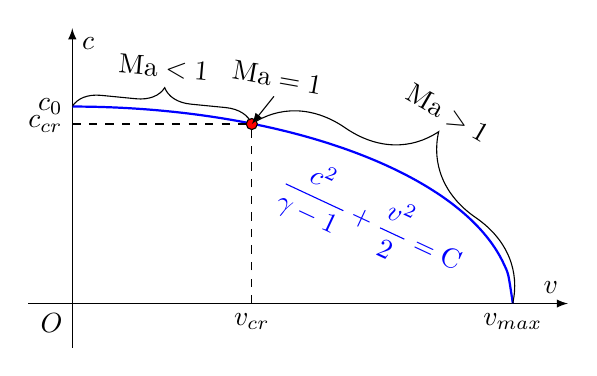
\begin{tikzpicture}
      \begin{axis}[
        axis equal image,
        axis lines=middle,
        axis line style={-latex},
        xmin = -0.4, xmax = 4.5,
        ymin = -0.4, ymax = 2.5,
        xtick=\empty,
        ytick=\empty,
        xlabel={$v$},
        ylabel={$c$},
        %title={$c$-$v$曲线平面图},
        ]
        \addplot[smooth, samples=100,domain=0:4, thick, blue] {(3.2-0.2*x^2)^(0.5)};
        \draw[dashed] (axis cs:1.63,0) node[anchor=north]{$v_{cr}$} -- (axis cs:1.63,1.63)
          node(cr)[xshift=8pt,yshift=10pt,rotate=-10,anchor=south]{$\mathrm{Ma}=1$};
        \draw[dashed] (axis cs:0,1.63) node[anchor=east]{$c_{cr}$} -- (axis cs:1.63,1.63);
        \draw (axis cs:0,1.79) node[anchor=east]{$c_{0}$};
        \node at (axis cs:4,0) [anchor=north]{$v_{max}$};
        \node at (axis cs:0,0) [anchor=north east] {$O$};
        \draw[decorate,decoration={brace, amplitude=10pt}] (axis cs:0,1.79)
          --node[midway, yshift=10pt,rotate=-5,anchor=south]{$\mathrm{Ma}<1$}
          (axis cs:1.63,1.63);
        \draw[decorate,decoration={brace, amplitude=36pt}] (axis cs:1.63,1.63)
          --node[midway, xshift=20pt,yshift=30pt,rotate=-30,anchor=south]{$\mathrm{Ma}>1$}
          (axis cs:4,0);
        \draw[fill=red] (axis cs:1.63,1.63) circle (2pt);
        \draw[-latex] (cr.south) -- (axis cs:1.63,1.63);
        \draw[blue] (axis cs:2,1.5) node[rotate=-25,anchor=north west] {$\displaystyle \frac{c^{2}}{\gamma-1}+\frac{v^{2}}{2}=\mathrm{C}$};
      \end{axis}
    \end{tikzpicture}
  \end{center}
  \begin{definition}[临界状态]
    一维定常等熵气流的某一截面上的速度等于当地声速时的状态称为临界状态。用下标
    $cr$表示。临界状态下的气流参数称为临界参数,该截面为临界截面。
  \end{definition}
\end{frame}

\begin{frame}{临界状态——续}
 临界状态下:
 \begin{equation*}
   v_{cr}
   =
   c_{cr}
 \end{equation*}
 \begin{equation*}
   \frac{c_{cr}^{2}}{\gamma-1}
   +
   \frac{v_{cr}^{2}}{2}
   =
   \frac{c_{0}^{2}}{\gamma-1}
   =
   \frac{v_{max}^{2}}{2}
 \end{equation*}
 \begin{equation*}
   c_{cr}
   =
   \sqrt{\gamma RT_{cr}}
   =
   \sqrt{\frac{2}{\gamma+1}}c_{0}
   =
   \sqrt{\frac{2\gamma R}{\gamma+1}T_{0}}
   =
   \sqrt{\frac{\gamma-1}{\gamma+1}}v_{max}
 \end{equation*}
 \vspace*{-1em}
 \only<2->{
 \begin{block}{讨论}
   \begin{itemize}
     \item<2-|alert@2> 对于给定气流运动,$c_{cr}$只取决于$T_{0}$
     \item<3-|alert@3> 在绝热流动中,$T_{0}$为常数,$c_{cr}$也是常数
     \item<4-|alert@4> 当地声速$c$是气体所处状态下实际存在的声速;临界声速$c_{cr}$是与气流所处状态相对应的临界状态下的声速
     \item<5-|alert@5> 当$\mathrm{Ma}=1$时,当地声速就是临界声速
   \end{itemize}
 \end{block}
 }
\end{frame}

\subsection{一维定常等熵气流中各参数关系式}
\subsubsection{以马赫数$\mathrm{Ma}$为变量的各参数关系式}
\begin{frame}{以马赫数$\mathrm{Ma}$为变量的各参数关系式}
  \vspace*{-1em}
  \begin{equation*}
    h
    +
    \frac{v^{2}}{2}
    =
    h_{0}
    \quad\quad
    c_{p}T
    +
    \frac{v^{2}}{2}
    =
    c_{p}T_{0}
    \quad\quad
    \frac{c^{2}}{\gamma-1}
    +
    \frac{v^{2}}{2}
    =
    \frac{c_{0}^{2}}{\gamma-1}
  \end{equation*}
  %\begin{equation*}
    %h
    %=
    %c_{p}T
  %\end{equation*}
  %\begin{equation*}
    %c_{p}
    %=
    %\frac{\gamma}{\gamma-1}R
  %\end{equation*}
  %\begin{equation*}
  %c
  %=
  %\sqrt{\gamma RT}
  %\end{equation*}
  %\begin{equation*}
    %\mathrm{Ma}
    %=
    %\frac{v}{c}
  %\end{equation*}
  \begin{equation*}
    \frac{T_{0}}{T}
    =
    \frac{c_{0}^{2}}{c^{2}}
    =
    1
    +
    \frac{\gamma-1}{2}\mathrm{Ma}^{2}
  \end{equation*}
  由等熵过程关系式:
  \begin{equation*}
    \frac{p}{\rho^{\gamma}}
    =
    \mathrm{C}
    \quad
    \rightarrow
    \quad
    \frac{p_{0}}{p}
    =
    \left(\frac{\rho_{0}}{\rho}\right)^{\gamma}
    =
    \left(\frac{T_{0}}{T}\right)^{\frac{\gamma}{\gamma-1}}
  \end{equation*}
  \begin{equation*}
    \frac{p_{0}}{p}
    =
    \left(1+\frac{\gamma-1}{2}\mathrm{Ma}^{2}\right)^{\frac{\gamma}{\gamma-1}}
  \end{equation*}
  \begin{equation*}
    \frac{\rho_{0}}{\rho}
    =
    \left(1+\frac{\gamma-1}{2}\mathrm{Ma}^{2}\right)^{\frac{1}{\gamma-1}}
  \end{equation*}
\end{frame}

\subsubsection{以速度系数$M_{*}$为变量的各参数关系式}
\begin{frame}{以速度系数$M_{*}$为变量的各参数关系式}
  \begin{itemize}
    \item 速度系数$M_{*}$表示气流速度与临界声速之比
      \begin{equation*}
        M_{*}
        =
        \frac{v}{c_{cr}}
      \end{equation*}
  \end{itemize}
  \vspace*{-1.5em}
  \begin{columns}[c]
    \begin{column}{0.45\textwidth}
  \begin{equation*}
    \frac{c^{2}}{\gamma-1}
    +
    \frac{v^{2}}{2}
    =
    \frac{c_{cr}^{2}}{\gamma-1}
    +
    \frac{c_{cr}^{2}}{2}
  \end{equation*}
  \begin{equation*}
    \frac{1}{\gamma-1}\frac{1}{\mathrm{Ma}^{2}}
    +
    \frac{1}{2}
    =
    \frac{\gamma+1}{2(\gamma-1)}\frac{1}{M_{*}^{2}}
  \end{equation*}
  \begin{equation*}
    M_{*}^{2}
    =
    \frac{(\gamma+1)\mathrm{Ma}^{2}}{2+(\gamma-1)\mathrm{Ma}^{2}}
  \end{equation*}
  \begin{equation*}
    \mathrm{Ma}^{2}
    =
  \frac{2M_{*}^{2}}{(\gamma+1)+(\gamma-1)M_{*}^{2}}
  \end{equation*}
    \end{column}
  
    \begin{column}{0.55\textwidth}
      \begin{center}
        \adjustbox{width=7cm}{
          % To Do
      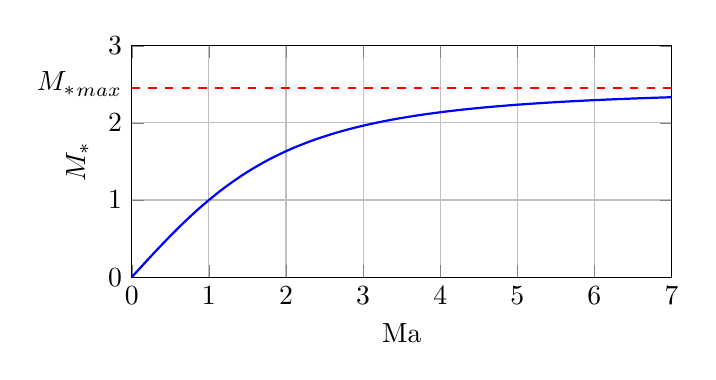
\begin{tikzpicture}
        \begin{axis}[
          axis equal image,
          xmin = 0, xmax = 7,
          ymin = 0, ymax = 3,
          xlabel={$\mathrm{Ma}$},
          ylabel={$M_{*}$},
          grid,
          ]
          \addplot[domain=0:7,smooth,thick,blue]{sqrt((2.4*x^2)/(2+0.4*x^2))};
          \addplot[domain=0:7,dashed,thick,red]{sqrt(6)};
        \end{axis}
          \node at (0,2.45) [anchor=east] {${M_{*}}_{max}$};
      \end{tikzpicture}
    }
      \end{center}
    \end{column}
  \end{columns}
\end{frame}

\begin{frame}{$M_{*}$表示的各参数关系式——续}
  \vspace*{-1.5em}
 \begin{equation*}
   \frac{T}{T_{0}}
   =
   \frac{c^{2}}{c_{0}^{2}}
   =
   1
   -
   \frac{\gamma-1}{\gamma+1}M_{*}^{2}
 \end{equation*} 
 \begin{equation*}
   \frac{p}{p_{0}}
   =
   \left(1-\frac{\gamma-1}{\gamma+1}M_{*}^{2}\right)^{\frac{\gamma}{\gamma-1}}
 \end{equation*}
 \begin{equation*}
   \frac{\rho}{\rho_{0}}
   =
   \left(1-\frac{\gamma-1}{\gamma+1}M_{*}^{2}\right)^{\frac{1}{\gamma-1}}
 \end{equation*}
  \vspace*{-1.5em}
 \begin{block}{讨论}
   \begin{enumerate}
     \item 使用$M_{*}$计算气流速度$v$比使用$\mathrm{Ma}$方便
     \item 在极限状态下,$\mathrm{Ma}=\infty$,
     $M_{*}=v_{max}/c_{cr}=\sqrt{(\gamma+1)/(\gamma-1)}$
     \item $M_{*}$也可作为流动类型的判别标准
       \begin{itemize}
         \item $\mathrm{Ma}<1$,$M_{*}<1$,亚声速流
         \item $\mathrm{Ma}=1$,$M_{*}=1$,声速流
         \item $\mathrm{Ma}>1$,$M_{*}>1$,超声速流
       \end{itemize}
   \end{enumerate}
 \end{block}
\end{frame}

\begin{frame}{临界参数与滞止参数的关系式}
  \vspace*{-1.5em}
  \begin{equation*}
    \left\{
      \begin{aligned}
    \frac{T_{0}}{T}
    &=
    1+\frac{\gamma-1}{2}\mathrm{Ma}^{2}
    \\
    \frac{p_{0}}{p}
    &=
    \left(1+\frac{\gamma-1}{2}\mathrm{Ma}^{2}\right)^{\frac{\gamma}{\gamma-1}}
    \\
    \frac{\rho_{0}}{\rho}
    &=
    \left(1+\frac{\gamma-1}{2}\mathrm{Ma}^{2}\right)^{\frac{1}{\gamma-1}}
      \end{aligned}
    \right.
    \xrightarrow{
      \mathrm{Ma}=1
  }
    \left\{
    \begin{aligned}
    \frac{T_{cr}}{T_{0}}
    &=
    \frac{c_{cr}^{2}}{c_{0}^{2}}
    =
    \frac{2}{\gamma+1}
    \\
    \frac{p_{cr}}{p_{0}}
    &=
    \left(\frac{2}{\gamma+1}\right)^{\frac{\gamma}{\gamma-1}}
    \\
    \frac{\rho_{cr}}{\rho_{0}}
    &=
    \left(\frac{2}{\gamma+1}\right)^{\frac{1}{\gamma-1}}
    \end{aligned}
    \right.
  \end{equation*}
  \vspace*{-1.5em}
  \begin{block}{讨论}
    \begin{itemize}
      %\item 临界参数与滞止参数的比值时常数
      \item 若$\gamma=1.4$,$\displaystyle \frac{T_{cr}}{T_{0}}=0.8333$,
        $\displaystyle \frac{p_{cr}}{p_{0}}=0.5283$,$\displaystyle
        \frac{\rho_{cr}}{\rho_{0}}=0.6339$,声速流动
      \item 若$\displaystyle \frac{T}{T_{0}}>0.8333$,
        $\displaystyle \frac{p}{p_{0}}>0.5283$,$\displaystyle
        \frac{\rho}{\rho_{0}}>0.6339$,亚声速流动
      \item 若$\displaystyle \frac{T}{T_{0}}<0.8333$,
        $\displaystyle \frac{p}{p_{0}}<0.5283$,$\displaystyle
        \frac{\rho}{\rho_{0}}<0.6339$,超声速流动
    \end{itemize}
  \end{block}
\end{frame}

\begin{frame}{各参数关系式示例}
  \vspace*{-0.5em}
  \begin{block}{例:气体在一无摩擦的渐缩管道中流动,已知截面1的压强为
      $p_{1}=2.67\times10^{5}\mathrm{Pa}$,温度为$T_{1}=330\mathrm{K}$,流速为
      $v_{1}=157\mathrm{m/s}$,并且在管道出口截面2达到临界状态。试求气流在出口截
      面的压强、密度、温度和速度。假定气体为空气,$\gamma=1.4$,
      $R=287\mathrm{J/(kg\cdot K)}$。
   }
   \only<2>{解: 首先计算截面1的声速$c_{1}$,马赫数$\mathrm{Ma}_{1}$,滞止压强$p_{0}$和滞
   止温度$T_{0}$
   \vspace{-0.5em}
   \begin{equation*}
     c_{1}
     =
     \sqrt{\gamma RT_{1}}
     =
     \sqrt{1.4\times287\times330}
     =
     364.1\mathrm{m/s}
   \end{equation*}
   \begin{equation*}
     \mathrm{Ma}_{1}
     =
     \frac{v_{1}}{c_{1}}
     =
     \frac{157}{364.1}
     =
     0.4312
   \end{equation*}
   \begin{equation*}
     \frac{T_{0}}{T_{1}}
     =
     1+\frac{\gamma-1}{2}\mathrm{Ma}_{1}^{2}
     =
     1 + \frac{1.4-1}{2}\times0.4312^{2}
     =
     1.037
   \end{equation*}
   \begin{equation*}
     T_{0}
     =
     T_{1}
     \left(1+\frac{\gamma-1}{2}\mathrm{Ma}_{1}^{2}\right)
     =
     330\times1.037
     =
     342.3\mathrm{K}
   \end{equation*}
 }
 \only<3>{
   \begin{equation*}
   \frac{\gamma}{\gamma-1}
   =
   \frac{1.4}{1.4-1}
   =
   3.5
   \end{equation*}
   \begin{equation*}
     p_{0}
     =
     p_{1}
     \left(1+\frac{\gamma-1}{2}\mathrm{Ma}_{1}^{2}\right)^{\frac{\gamma}{\gamma-1}}
     =
     2.67\times10^{5}\times1.037^{3.5}
     =
     3.034\times10^{5}\mathrm{Pa}
   \end{equation*}
   \begin{equation*}
   \frac{2}{\gamma+1}
   =
   \frac{2}{1.4+1}
   =
   0.833
   \end{equation*}
   \begin{equation*}
     p_{2}
     =
     p_{cr}
     =
     p_{0}\left(\frac{2}{\gamma+1}\right)^{\frac{\gamma}{\gamma-1}}
     =
     3.034\times10^{5}\times0.833^{3.5}
     =
     1.411\times10^{5}\mathrm{Pa}
   \end{equation*}
 }
 \only<4>{
   \begin{equation*}
     T_{2}
     =
     T_{cr}
     =
     T_{0}\frac{2}{\gamma+1}
     =
     342.3\times0.833
     =
     285.25\mathrm{K}
   \end{equation*}
   \begin{equation*}
     \rho_{2}
     =
     \rho_{cr}
     =
     \frac{p_{cr}}{RT_{cr}}
     =
     \frac{1.411\times10^{5}}{287\times285.25}
     =
     1.724\mathrm{kg/m^{3}}
   \end{equation*}
   \begin{equation*}
     v_{2}
     =
     c_{cr}
     =
     \sqrt{\gamma RT_{cr}}
     =
     \sqrt{1.4\times287\times285.25}
     =
     338.5\mathrm{m/s}
   \end{equation*}
 }
 \end{block} 
\end{frame}
